%
%このファイルは日本バーチャルリアリティ学会論文集用スタイルファイル
%jvrst2e.sty(ver.2.0) を利用したサンプルファイルです。

\documentclass[a4paper,twoside]{jarticle}
   \usepackage{style/tvrsj2e}
   % \usepackage[dvips]{graphicx}
   \usepackage[dvipdfmx]{graphicx}
   \usepackage{style/listings,style/jlisting} %日本語のコメントアウトをする場合jlistingが必要
   \usepackage{here}
   \usepackage{amsmath}

%和文タイトル 論文のヘッダ部分にも出力されます。 
\jtitle{
    計算物理演習レポート2 数値計算}

%著者日本名
\jauthor{}

% ヘッダー
\header{計算物理演習レポート2 数値計算}

%論文の種別に合わせる
\TYPE{レポート}
%\TYPE{基礎論文}
%\TYPE{応用論文}
%\TYPE{コンテンツ論文}
%\TYPE{総説論文}
%\TYPE{ショートペーパー}

%ここからソースコードの表示に関する設定
\lstset{
  basicstyle={\ttfamily},
  identifierstyle={\small},
  commentstyle={\smallitshape},
  keywordstyle={\small\bfseries},
  ndkeywordstyle={\small},
  stringstyle={\small\ttfamily},
  frame={tb},
  breaklines=true,
  columns=[l]{fullflexible},
  numbers=left,
  xrightmargin=0zw,
  xleftmargin=3zw,
  numberstyle={\scriptsize},
  stepnumber=1,
  numbersep=1zw,
  lineskip=-0.5ex
}
%ここまでソースコードの表示に関する設定

\begin{document}

%maketitle は abstract と keyword の後に入れてください。

\maketitle

\section{概要}
2体問題の数値計算を行った。数値計算の手法としては、Euler 法、Leapfrog 法、古典4次 Runge-Kutta 法を用いた。また、各値の計算には C++ 14、プロットには gnuplot を使用した。

\section{Euler 法}\label{s-euler}

\subsection{内容}
2体問題の数値計算を Euler 法で行った。

また、力学的エネルギーもプロットを行った。力学的エネルギーは
\begin{align}
  E(t)=\frac{1}{2}mv(t)^2-\frac{GMm}{r(t)}
\end{align}
で表される。これの理論値($t=0$での値)と各時間での値を比較した。

\subsection{ソースコード}
euler/n.cpp
% \begin{lstlisting}[caption=hoge,label=fuga]
% \begin{figure}[t]
\begin{lstlisting}[]
#include <string>
#include "../../util.h"

using namespace std;

int main() {
    const double dt = 0.1, G = 1.0, M = 1.0, m = 1.0;
    int n = 2000;
    double x[n], y[n], v_x[n], v_y[n];
    x[0] = 0.5, y[0] = 0.0, v_x[0] = 0.0, v_y[0] = 1.63;
    for (int i = 0; i < n - 1; i++) {
        x[i + 1] = x[i] + v_x[i] * dt;
        y[i + 1] = y[i] + v_y[i] * dt;
        double r = sqrt(pow(x[i], 2) + pow(y[i], 2));
        v_x[i + 1] = v_x[i] - G * M * m * x[i] / (pow(r, 3) * m) * dt;
        v_y[i + 1] = v_y[i] - G * M * m * y[i] / (pow(r, 3) * m) * dt;
    }
    string s;
    for (int i = 0; i < n; i++) {
        s += to_string(x[i]) + " " + to_string(y[i]) + "\n";
    }
    string fpath = "../out/euler/n.dat";
    write_to_file(s, fpath);

//    gnuplot で
//    ```set size ratio -1
//       plot 'n.dat' with points pointtype 0```
//    でプロット
    return 0;
}
\end{lstlisting}
% \end{figure}

util.cpp
\begin{lstlisting}
//#include <random>
#include "Sample.h"

using namespace std;
\end{lstlisting}

util.h
\begin{lstlisting}
#pragma once

#include <fstream>
#include <random>

using namespace std;

inline double get_random_0_to_1() {
  // 乱数生成器
  static mt19937_64 mt64(0);

  // [0.0, 1.0) の一様分布実数生成器
  uniform_real_distribution<double> get_rand_uni_real(0.0, 1.0);
  // 乱数を生成
  return get_rand_uni_real(mt64);
}

inline int write_to_file(const string& s, const string& fpath) {
  ofstream f;
  f.open(fpath);
  f << s;
  f.close();
  return 0;
}
\end{lstlisting}

\subsection{結果}

\begin{figure}[H]
\begin{center}
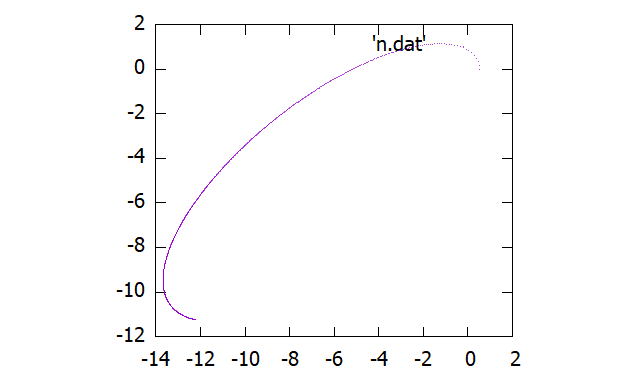
\includegraphics[width=8cm]{../cpp/out/euler/euler_dt=e-1_n=1000.png}
\end{center}
\caption{$\mathrm{d}t=0.1, \mathrm{n}=1000$とした場合}
\end{figure}

$\mathrm{d}t$は$0.1$のまま、nをもう少し大きくしたとき(5000秒先まで追ったとき)

\begin{figure}[H]
\begin{center}
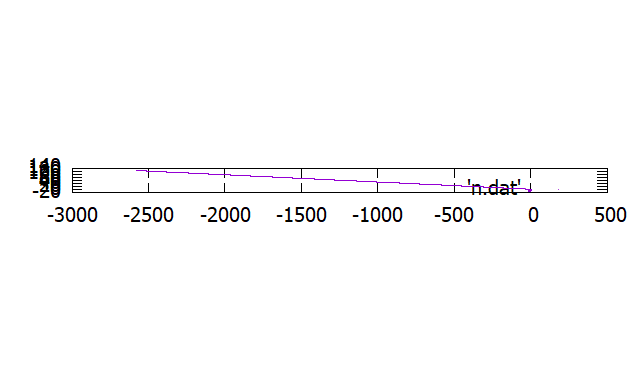
\includegraphics[width=8cm]{../cpp/out/euler/euler_dt=e-1_n=50000.png}
\end{center}
\caption{$\mathrm{d}t=0.1, \mathrm{n}=50000$とした場合}
\end{figure}

$\mathrm{d}t$は$0.1$のまま、nを少しだけ大きくしたとき(200秒先まで追ったとき)

\begin{figure}[H]
\begin{center}
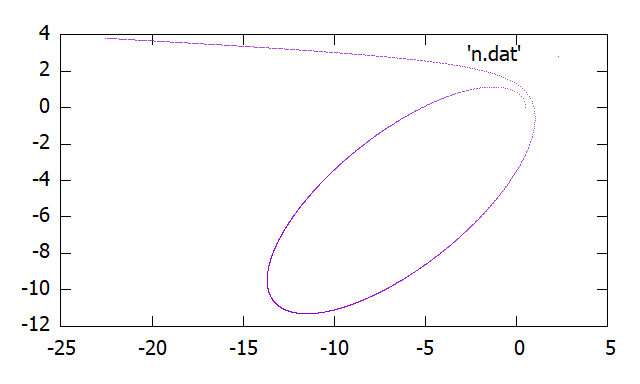
\includegraphics[width=8cm]{../cpp/out/euler/euler_dt=e-1_n=2000.png}
\end{center}
\caption{$\mathrm{d}t=0.1, \mathrm{n}=2000$とした場合}
\end{figure}

\begin{figure}[H]
$\mathrm{d}t$をもう少し小さくしたとき($\mathrm{d}t=0.01$で時刻は同じ200秒まで)
\begin{center}
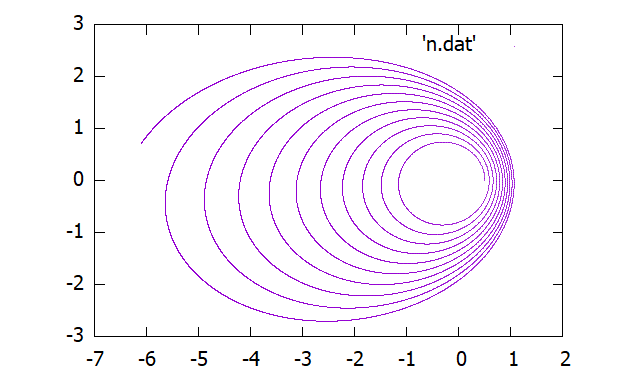
\includegraphics[width=8cm]{../cpp/out/euler/euler_dt=e-2_n=20000.png}
\end{center}
\caption{$\mathrm{d}t=0.01, \mathrm{n}=20000$とした場合}
\end{figure}

\begin{figure}[H]
力学的エネルギーの時間変化
\begin{center}
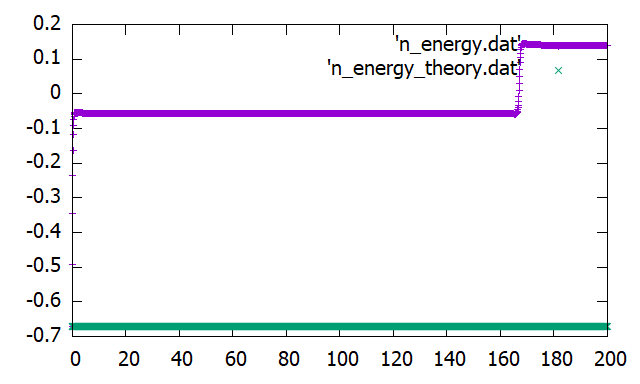
\includegraphics[width=8cm]{../cpp/out/euler/n_energy.png}
\end{center}
\caption{力学的エネルギーの時間変化(t=200まで)}
\end{figure}

\subsection{考察}
徐々に半径が変わっているが、これはEuler法がエネルギーを保存しないためと考えられる。また、$\mathrm{d}t$を小さくすればより精度が高くなっているが、これは$\frac{\Delta x}{\Delta t}$を小さくすればより$\displaystyle \frac{\mathrm{d}x}{\mathrm{d}t}=\lim_{\Delta t \to 0}\frac{\Delta x}{\Delta t}$に近づくためと考えられる。

また、力学的エネルギーは常に一定の値をとる理論値と比べて、計算した値は増加している。これは、Euler法がエネルギーを保存しないためと考えられる。

\section{Leapfrog法}
\subsection{内容}
同じ2体問題の数値計算をLeapfrog法でも行った。

\subsection{ソースコード}
leap-frog/n.cpp
\begin{lstlisting}
#include <string>
#include "../../util.h"

using namespace std;

int main() {
    const int tmax = 100;
    const int n = 1000;
    const double dt = double(tmax) / double(n), G = 1.0, M = 1.0, m = 1.0;
    double x[2 * n], y[2 * n], v_x[2 * n], v_y[2 * n];
    x[0] = 0.5, y[0] = 0.0, v_x[0] = 0.0, v_y[0] = 1.63;

    double r = sqrt(pow(x[0], 2) + pow(y[0], 2));
    v_x[1] = v_x[0] - G * M * m * x[0] / (pow(r, 3) * m) * dt * 0.5;
    v_y[1] = v_y[0] - G * M * m * y[0] / (pow(r, 3) * m) * dt * 0.5;
    for (long i = 0; i < n - 1; i++) {
        x[2 * (i + 1)] = x[2 * i] + v_x[2 * i + 1] * dt;
        y[2 * (i + 1)] = y[2 * i] + v_y[2 * i + 1] * dt;
        r = sqrt(pow(x[2 * (i + 1)], 2) + pow(y[2 * (i + 1)], 2));
        v_x[2 * i + 3] = v_x[2 * i + 1] - G * M * m * x[2 * (i + 1)] / (pow(r, 3) * m) * dt;
        v_y[2 * i + 3] = v_y[2 * i + 1] - G * M * m * y[2 * (i + 1)] / (pow(r, 3) * m) * dt;
    }
    string s;
    for (int i = 0; i < n; i++) {
        s += to_string(x[2 * i]) + " " + to_string(y[2 * i]) + "\n";
    }
    string fpath = "../out/leap-frog/n.dat";
    write_to_file(s, fpath);

//    gnuplot で
//    ```set size ratio -1
//       plot 'n.dat' with points pointtype 0```
//    でプロット
    return 0;
}
\end{lstlisting}

util.h、util.cpp は\ref{s-euler}と同一である。

\subsection{結果}
\begin{figure}[H]
\begin{center}
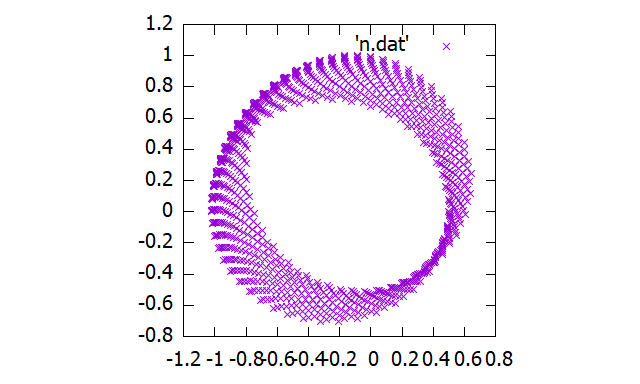
\includegraphics[width=8cm]{../cpp/out/leap-frog/n.png}
\end{center}
\caption{$\mathrm{d}t=0.1, \mathrm{n}=1000, v_y=1.63$とした場合}
\end{figure}

\begin{figure}[H]
$\mathrm{d}t$は$0.1$のまま、nをもう少し大きくしたとき(5000秒先まで追ったとき)
\begin{center}
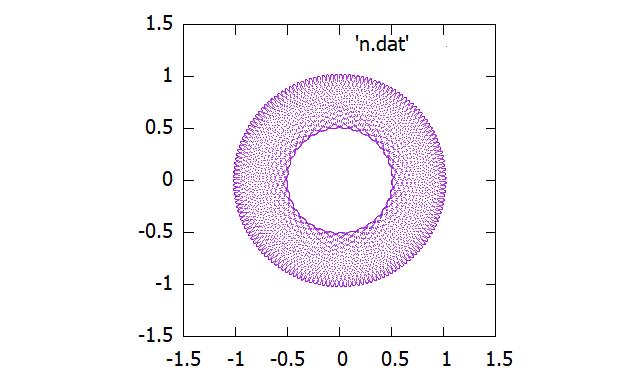
\includegraphics[width=8cm]{../cpp/out/leap-frog/n_dt=e-1_n=50000.png}
\end{center}
\caption{$\mathrm{d}t=0.1, \mathrm{n}=50000, v_y=1.63$とした場合}
\end{figure}

\begin{figure}[H]
力学的エネルギーの時間変化
\begin{center}
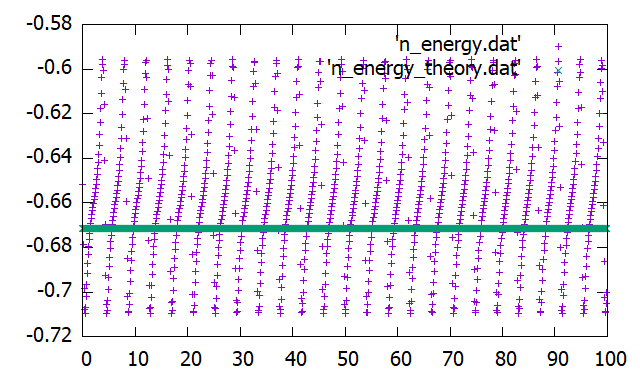
\includegraphics[width=8cm]{../cpp/out/leap-frog/n_energy_theory.png}
\end{center}
\caption{力学的エネルギーの時間変化(t=100まで)}
\end{figure}

\subsection{考察}
Euler法と違いLeapfrog法はエネルギーを保存するので、円の半径はほぼ一定に保たれているように見える。

実際、力学的エネルギーの理論値と計算結果との誤差をプロットしてみると、

\begin{figure}[H]
\begin{center}
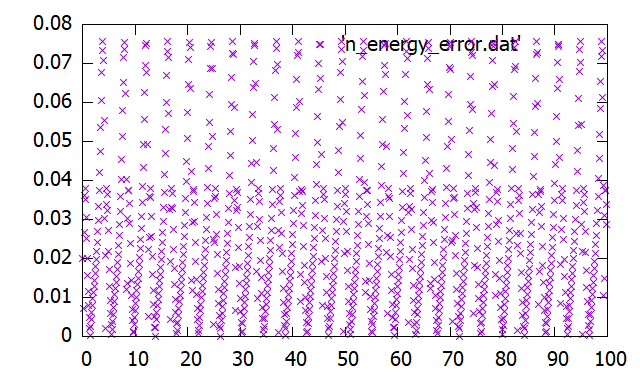
\includegraphics[width=8cm]{../cpp/out/leap-frog/n_error.png}
\end{center}
\caption{力学的エネルギーの誤差(理論値と計算結果の差)}
\end{figure}

と、誤差は一定の範囲内に保たれ、時間変化に渡って蓄積していかないことがわかる。これはLeapfrog法の持つシンプレクティック性による。

\section{古典4次 Runge-Kutta 法}
\subsection{内容}
テキストにはないが、同じ2体問題の数値計算を古典4次 Runge-Kutta 法(RK4)でも行った。

\subsection{計算方法}
運動方程式
\begin{align}
  m\frac{\mathrm{d}^2 x}{\mathrm{d}t^2}=-\frac{GMmx}{r^3}\\
  m\frac{\mathrm{d}^2 y}{\mathrm{d}t^2}=-\frac{GMmy}{r^3}
\end{align}
は次のような$x$、$y$、$v_x$、$v_y$についての連立常微分方程式で書ける。
\begin{align}
  \frac{\mathrm{d}x}{\mathrm{d}t}&=v_x&\\
  \frac{\mathrm{d}y}{\mathrm{d}t}&=v_y&\\
  \frac{\mathrm{d}v_x}{\mathrm{d}t}&=-\frac{GMmx}{mr^3}&\\
  \frac{\mathrm{d}v_y}{\mathrm{d}t}&=-\frac{GMmy}{mr^3}&
\end{align}
ここで、各方程式の右辺をそれぞれ
\begin{align}
  \frac{\mathrm{d}x}{\mathrm{d}t}&=f\left(t,x,y,v_x,v_y\right)&\\
  \frac{\mathrm{d}y}{\mathrm{d}t}&=g\left(t,x,y,v_x,v_y\right)&\\
  \frac{\mathrm{d}v_x}{\mathrm{d}t}&=h\left(t,x,y,v_x,v_y\right)&\\
  \frac{\mathrm{d}v_y}{\mathrm{d}t}&=i\left(t,x,y,v_x,v_y\right)&
\end{align}
と置くと、$t_{i+1}$、$x_{i+1}$、$y_{i+1}$、$v_{x_{i+1}}$、$v_{y_{i+1}}$は$t_{i}$、$x_{i}$、$y_{i}$、$v_{x_{i}}$、$v_{y_{i}}$を使って次のように求められる。
\begin{align}
  t_{i+1}&=t_{i}+\mathrm{d}t&\\
  x_{i+1}&=x_{i}+\frac{\mathrm{d}t}{6}\left(k_0+2k_1+2k_2+k_3\right)&\\
  y_{i+1}&=y_{i}+\frac{\mathrm{d}t}{6}\left(l_0+2l_1+2l_2+l_3\right)&\\
  v_{x_{i+1}}&=v_{x_{i}}+\frac{\mathrm{d}t}{6}\left(m_0+2m_1+2m_2+m_3\right)&\\
  v_{y_{i+1}}&=v_{y_{i}}+\frac{\mathrm{d}t}{6}\left(n_0+2n_1+2n_2+n_3\right)&
\end{align}
ただし、
\footnotesize
\begin{align}
  k_0&=f\left(t_i,x_i,y_i,v_{x_{i}},v_{y_{i}}\right)&\\
  l_0&=g\left(t_i,x_i,y_i,v_{x_{i}},v_{y_{i}}\right)&\\
  m_0&=h\left(t_i,x_i,y_i,v_{x_{i}},v_{y_{i}}\right)&\\
  n_0&=i\left(t_i,x_i,y_i,v_{x_{i}},v_{y_{i}}\right)&\\
  k_1&=f\left(t_i+\frac{\mathrm{d}t}{2},x_i+\frac{\mathrm{d}tk_0}{2},y_i+\frac{\mathrm{d}tl_0}{2},v_{x_{i}}+\frac{\mathrm{d}tm_0}{2},v_{y_{i}}+\frac{\mathrm{d}tn_0}{2}\right)&\\
  l_1&=g\left(t_i+\frac{\mathrm{d}t}{2},x_i+\frac{\mathrm{d}tk_0}{2},y_i+\frac{\mathrm{d}tl_0}{2},v_{x_{i}}+\frac{\mathrm{d}tm_0}{2},v_{y_{i}}+\frac{\mathrm{d}tn_0}{2}\right)&\\
  m_1&=h\left(t_i+\frac{\mathrm{d}t}{2},x_i+\frac{\mathrm{d}tk_0}{2},y_i+\frac{\mathrm{d}tl_0}{2},v_{x_{i}}+\frac{\mathrm{d}tm_0}{2},v_{y_{i}}+\frac{\mathrm{d}tn_0}{2}\right)&\\
  n_1&=i\left(t_i+\frac{\mathrm{d}t}{2},x_i+\frac{\mathrm{d}tk_0}{2},y_i+\frac{\mathrm{d}tl_0}{2},v_{x_{i}}+\frac{\mathrm{d}tm_0}{2},v_{y_{i}}+\frac{\mathrm{d}tn_0}{2}\right)&\\
  k_2&=f\left(t_i+\frac{\mathrm{d}t}{2},x_i+\frac{\mathrm{d}tk_1}{2},y_i+\frac{\mathrm{d}tl_1}{2},v_{x_{i}}+\frac{\mathrm{d}tm_1}{2},v_{y_{i}}+\frac{\mathrm{d}tn_1}{2}\right)&\\
  l_2&=g\left(t_i+\frac{\mathrm{d}t}{2},x_i+\frac{\mathrm{d}tk_1}{2},y_i+\frac{\mathrm{d}tl_1}{2},v_{x_{i}}+\frac{\mathrm{d}tm_1}{2},v_{y_{i}}+\frac{\mathrm{d}tn_1}{2}\right)&\\
  m_2&=h\left(t_i+\frac{\mathrm{d}t}{2},x_i+\frac{\mathrm{d}tk_1}{2},y_i+\frac{\mathrm{d}tl_1}{2},v_{x_{i}}+\frac{\mathrm{d}tm_1}{2},v_{y_{i}}+\frac{\mathrm{d}tn_1}{2}\right)&\\
  n_2&=i\left(t_i+\frac{\mathrm{d}t}{2},x_i+\frac{\mathrm{d}tk_1}{2},y_i+\frac{\mathrm{d}tl_1}{2},v_{x_{i}}+\frac{\mathrm{d}tm_1}{2},v_{y_{i}}+\frac{\mathrm{d}tn_1}{2}\right)&\\
  k_3&=f\left(t_i+\mathrm{d}t,x_i+\mathrm{d}tk_2,y_i+\mathrm{d}tl_2,v_{x_{i}}+\mathrm{d}tm_2,v_{y_{i}}+\mathrm{d}tn_2\right)&\\
  l_3&=g\left(t_i+\mathrm{d}t,x_i+\mathrm{d}tk_2,y_i+\mathrm{d}tl_2,v_{x_{i}}+\mathrm{d}tm_2,v_{y_{i}}+\mathrm{d}tn_2\right)&\\
  m_3&=h\left(t_i+\mathrm{d}t,x_i+\mathrm{d}tk_2,y_i+\mathrm{d}tl_2,v_{x_{i}}+\mathrm{d}tm_2,v_{y_{i}}+\mathrm{d}tn_2\right)&\\
  n_3&=i\left(t_i+\mathrm{d}t,x_i+\mathrm{d}tk_2,y_i+\mathrm{d}tl_2,v_{x_{i}}+\mathrm{d}tm_2,v_{y_{i}}+\mathrm{d}tn_2\right)&
\end{align}
\normalsize
である。

\subsection{ソースコード}
runge-kutta/n.cpp
\begin{lstlisting}
#include <string>
#include "../../util.h"

using namespace std;

#define tmax 100
#define n 1000
#define dt double(tmax) / double(n)
#define G 1.0
#define M 1.0
#define m 1.0

double f_dx_dt(double t, double _x, double _y, double _v_x, double _v_y) {
    return _v_x;
}

double g_dy_dt(double t, double _x, double _y, double _v_x, double _v_y) {
    return _v_y;
}

double h_dv_x_dt(double t, double _x, double _y, double _v_x, double _v_y) {
    double r = sqrt(pow(_x, 2) + pow(_y, 2));
    return -G * M * m * _x / (pow(r, 3) * m);
}

double i_dv_y_dt(double t, double _x, double _y, double _v_x, double _v_y) {
    double r = sqrt(pow(_x, 2) + pow(_y, 2));
    return -G * M * m * _y / (pow(r, 3) * m);
}

int main() {
    double t[n], x[n], y[n], v_x[n], v_y[n];
    t[0] = 0.0, x[0] = 0.5, y[0] = 0.0, v_x[0] = 0.0, v_y[0] = 1.63;

    for (int i = 0; i < n - 1; i++) {
        double k0 = f_dx_dt(t[i], x[i], y[i], v_x[i], v_y[i]);
        double l0 = g_dy_dt(t[i], x[i], y[i], v_x[i], v_y[i]);
        double m0 = h_dv_x_dt(t[i], x[i], y[i], v_x[i], v_y[i]);
        double n0 = i_dv_y_dt(t[i], x[i], y[i], v_x[i], v_y[i]);
        double k1 = f_dx_dt(t[i] + dt / 2.0, x[i] + dt / 2.0 * k0, y[i] + dt / 2.0 * l0, v_x[i] + dt / 2.0 * m0, v_y[i] + dt / 2.0 * n0);
        double l1 = g_dy_dt(t[i] + dt / 2.0, x[i] + dt / 2.0 * k0, y[i] + dt / 2.0 * l0, v_x[i] + dt / 2.0 * m0, v_y[i] + dt / 2.0 * n0);
        double m1 = h_dv_x_dt(t[i] + dt / 2.0, x[i] + dt / 2.0 * k0, y[i] + dt / 2.0 * l0, v_x[i] + dt / 2.0 * m0, v_y[i] + dt / 2.0 * n0);
        double n1 = i_dv_y_dt(t[i] + dt / 2.0, x[i] + dt / 2.0 * k0, y[i] + dt / 2.0 * l0, v_x[i] + dt / 2.0 * m0, v_y[i] + dt / 2.0 * n0);
        double k2 = f_dx_dt(t[i] + dt / 2.0, x[i] + dt / 2.0 * k1, y[i] + dt / 2.0 * l1, v_x[i] + dt / 2.0 * m1, v_y[i] + dt / 2.0 * n1);
        double l2 = g_dy_dt(t[i] + dt / 2.0, x[i] + dt / 2.0 * k1, y[i] + dt / 2.0 * l1, v_x[i] + dt / 2.0 * m1, v_y[i] + dt / 2.0 * n1);
        double m2 = h_dv_x_dt(t[i] + dt / 2.0, x[i] + dt / 2.0 * k1, y[i] + dt / 2.0 * l1, v_x[i] + dt / 2.0 * m1, v_y[i] + dt / 2.0 * n1);
        double n2 = i_dv_y_dt(t[i] + dt / 2.0, x[i] + dt / 2.0 * k1, y[i] + dt / 2.0 * l1, v_x[i] + dt / 2.0 * m1, v_y[i] + dt / 2.0 * n1);
        double k3 = f_dx_dt(t[i] + dt, x[i] + dt * k2, y[i] + dt * l2, v_x[i] + dt * m2, v_y[i] + dt * n2);
        double l3 = g_dy_dt(t[i] + dt, x[i] + dt * k2, y[i] + dt * l2, v_x[i] + dt * m2, v_y[i] + dt * n2);
        double m3 = h_dv_x_dt(t[i] + dt, x[i] + dt * k2, y[i] + dt * l2, v_x[i] + dt * m2, v_y[i] + dt * n2);
        double n3 = i_dv_y_dt(t[i] + dt, x[i] + dt * k2, y[i] + dt * l2, v_x[i] + dt * m2, v_y[i] + dt * n2);
        t[i + 1] = t[i] + dt;
        x[i + 1] = x[i] + (dt / 6.0) * (k0 + 2.0 * k1 + 2.0 * k2 + k3);
        y[i + 1] = y[i] + (dt / 6.0) * (l0 + 2.0 * l1 + 2.0 * l2 + l3);
        v_x[i + 1] = v_x[i] + (dt / 6.0) * (m0 + 2.0 * m1 + 2.0 * m2 + m3);
        v_y[i + 1] = v_y[i] + (dt / 6.0) * (n0 + 2.0 * n1 + 2.0 * n2 + n3);
    }
    string s;
    for (int i = 0; i < n; i++) {
        s += to_string(x[i]) + " " + to_string(y[i]) + "\n";
    }
    string fpath = "../out/runge-kutta/n.dat";
    write_to_file(s, fpath);

//    gnuplot で
//    ```set size ratio -1
//       plot 'n.dat' with points pointtype 0```
//    でプロット
    return 0;
}

\end{lstlisting}

util.h、util.cpp は\ref{s-euler}と同一である。

\subsection{結果}
\begin{figure}[H]
\begin{center}
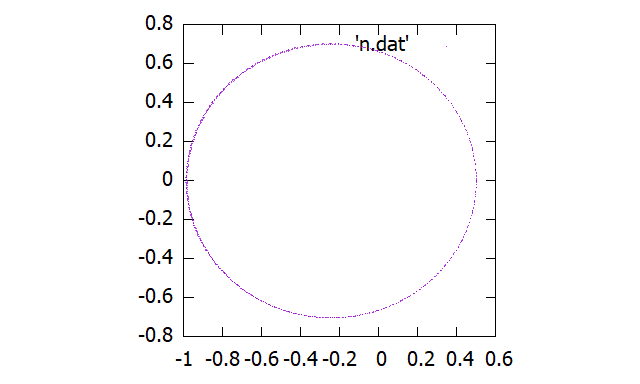
\includegraphics[width=8cm]{../cpp/out/runge-kutta/n.png}
\end{center}
\caption{$\mathrm{d}t=0.1, \mathrm{n}=1000, v_y=1.63$とした場合}
\end{figure}

\begin{figure}[H]
$\mathrm{d}t$は$0.1$のまま、nをもう少し大きくしたとき(5000秒先まで追ったとき)
\begin{center}
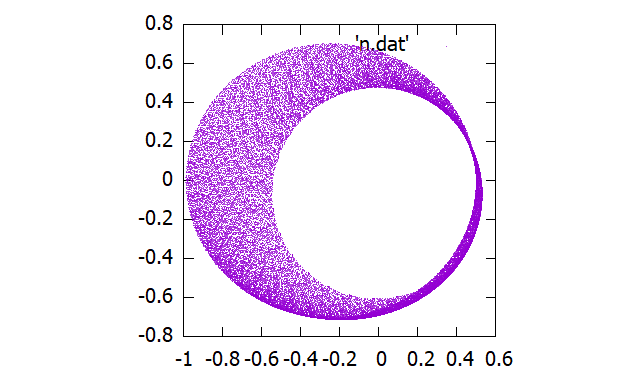
\includegraphics[width=8cm]{../cpp/out/runge-kutta/n_dt=e-1_n=50000.png}
\end{center}
\caption{$\mathrm{d}t=0.1, \mathrm{n}=50000, v_y=1.63$とした場合}
\end{figure}

\begin{figure}[H]
力学的エネルギーの時間変化(t=100まで))
\begin{center}
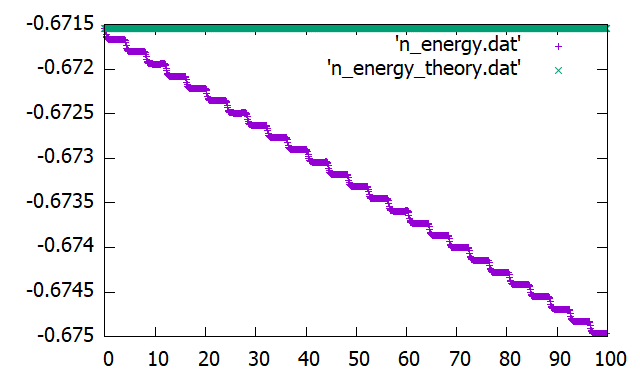
\includegraphics[width=8cm]{../cpp/out/runge-kutta/n_energy.png}
\end{center}
\caption{力学的エネルギーの時間変化(t=100まで)}
\end{figure}

\subsection{考察}
古典4次 Runkge-Kutta 法は4次精度なので、Euler 法や Leapfrog 法に比べ同じ$\mathrm{d}t=0.1$でもかなり精度がよくなっており、軌道がほとんどずれていない。

ただし、5000秒先まで追うとどんどん軌道半径が小さくなってしまった。これは、ただ軌道半径がほぼ一定に保たれて位置がずれるだけのLeapfrog 法とは違って、古典4次 Runkge-Kutta 法がエネルギーを保存しないためと思われる。

実際、誤差(力学的エネルギーの理論値と計算した値の差)は

\begin{figure}[H]
\begin{center}
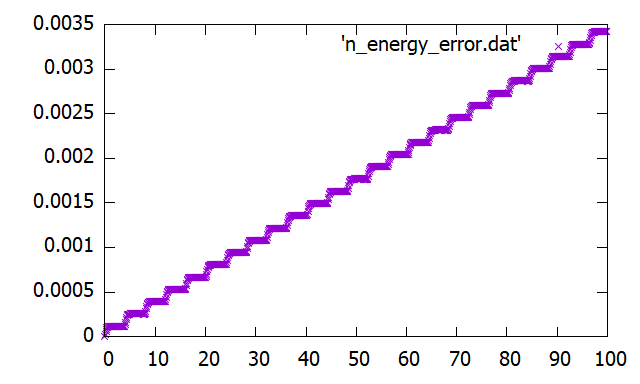
\includegraphics[width=8cm]{../cpp/out/runge-kutta/n_error.png}
\end{center}
\caption{力学的エネルギーの誤差(理論値と計算結果の差)}
\end{figure}

と、時間変化すると増加していくのがわかる。

\begin{thebibliography}{99}
\bibitem{sit}
ルンゲクッタ法による常微分方程式の数値解法 埼玉工業大学
https://www.sit.ac.jp/user/konishi/JPN/L\_Support/SupportPDF/Runge-KuttaMethod.pdf

\bibitem{wiki}
ルンゲ=クッタ法 - Wikipedia
https://ja.wikipedia.org/wiki/ルンゲ=クッタ法

\bibitem{naoj}
N 体シミュレーションの基礎 道越秀吾 国立天文台 CfCA
https://www.cfca.nao.ac.jp/~cfca/hpc/muv/text/michikoshi\_12.pdf

\bibitem{kagoshima}
suti-sekibun-bibun.pdf
https://www.sci.kagoshima-u.ac.jp/fujii/data\_kougi/suti-sekibun-bibun.pdf

\bibitem{qiita}
古典4次Runge-Kutta法の精度確認 - Qiita
https://qiita.com/kaityo256/items/e3428deb394b3ad1e739

\end{thebibliography}

\end{document}
